

\chapter{Methodology}

To calculate the flux of fireballs from our D6 AllSky Camera, we need to find the total observation area, time, and the total number of events.
In this section, we begin by describing in detail our methods for finding each of these properties.
Some time will be spend discussing obstacles such as camera fish-eye effect and cloud interference.  
Additionally, we will delve into the structure of our database: our fundamental tool for secondary statistical analysis.

\section{Calculating Total Observation Time}

Each night the D6 AllSky Camera observes, a program is run on the controlling Raspberry Pi that logs important information throughout the night.
The observation log is a simple time-stamped text file that records what processes the system runs at various times in a given night.
For instance, the observation log contains when each observation run begins (when the camera is set up initially), when the camera begins its analysis, when a new event is detected, and when the analysis goes to sleep, along with potential warnings or error messages that might come up.

To calculate the total observation time, we run a Python script that searches for the time associated with the start of each new analysis.  
After this time is recorded, we continue down the list of information until we find the time associated with that observation run's end.  
By subtracting the two times, we find the total observation time for that specific night.  
Performing this same method in a loop throughout all of the nights allows us to find how much time we spent observing on a given night. 
By summing up the total time observed over each night, we can attain the total observation time over the course of our data collection period.

A depiction of a portion of an observation log and our time analysis table can be seen in Figure~\ref{obslog_time}.
Note that while the information row that contains "New Observation Run Started" sounds as if it represents the start time, it does not.
A new observation run begins once the the D6 Camera is placed outside and turned on.  
Occasionally, the camera is set up while the sky is still too bright to begin actual video recordings. 
Therefore, we define our start time from a separate information row that states "A new night has arrived! Frame analysis beginning!". 
End times are determined by the information rows labeled "Day has come.  Analysis going to sleep."

\begin{figure}[ht!]
  \centering
  \includegraphics[scale=0.51]{images/obslog_time.png}
  \caption{An example observation log and the resulting time analysis information.}
  \label{obslog_time}
\end{figure}

Occasionally, we run tests on different D6 AllSky Camera actions. 
For example, we could program it to shut down, restart, or take pictures.
On August 29, 2018, one test resulted in no recorded "Day has come.  Analysis going to sleep." log.
This meant that we didn't have a correct log for that night's observation end time, leading to an error of a $14$ day observation session.
In actuality, the observation session was purely intended for testing and lasted less than one hour.  
Fringe cases like this raised red flags in our analysis and were looked at individually.
In all cases, these testing sessions were not considered part of our real observation.


It is imperative that we save not only the total observing time over a given night, but also the start and end times. 
This information is crucial for the next section, where we calculate the area of sky observed on a given night.

\section{Calculating Total Observation Area}

One of the most difficult problems we needed to address for this project was determining what area of the sky the D6 AllSky Camera observed each night.  
In an ideal world, our camera would be able to see all parts of the observable night sky, spanning across all horizons.  
However, due to optical limitations of our system and this is not possible.
Figure \ref{views_sidebyside} shows how our field of view is rectangular, as opposed to some other systems with a slightly more encompassing view.
This means that even if we new the total angular coverage of our camera with respect to the horizon, we wouldn't be able to precisely estimate our total observation area.
Nevertheless, determining the flux is a primary goal of this project, and is directly dependent on observation area. 

\begin{figure}[ht!]
  \makebox[\textwidth][c]{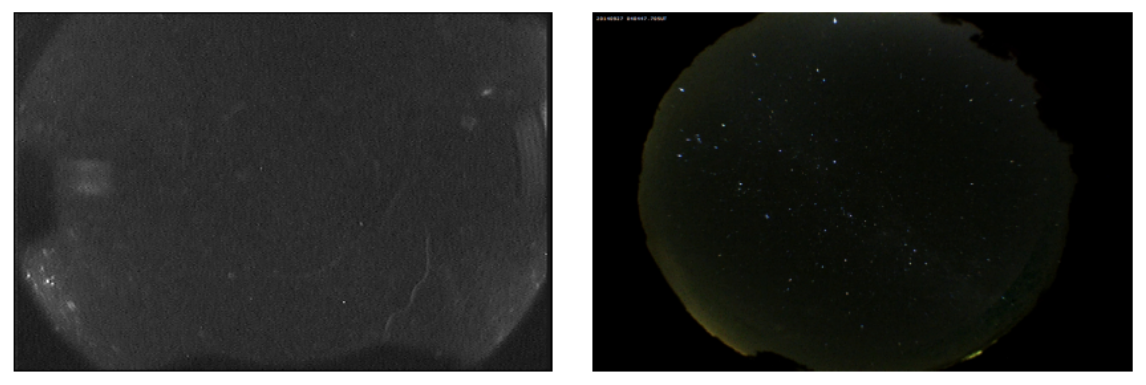
\includegraphics[width=1.0\textwidth]{images/allsky_view_sidebyside.png}}
  \caption{Left: our rectangular field of view.  Right:  A separate system's more complete circular view.}
  \label{views_sidebyside}
\end{figure}

To make matters more complicated, while the use of a fisheye lens gets us more coverage of the sky, it also results in some distortion of the image.
These distortions generally get worse the further an object is from is from zenith (directly overhead).
The significance of this problem as related to our project stems from the fact that while $50\% $ of our camera's pixels may be covered by clouds, this doesn't necessarily mean that $50\%$ of the observable sky is covered.
Therefore, we need some way of relating a given camera region to some observable distance.

To do this, we used observations of the Moon and various stars to calculate angular distance to pixel ratios for different regions of our camera.
This solution addresses the need to account for a camera fish-eye effect by assigning different fields-of-view to different pixel observational areas.
By correlating certain pixels with specific angular distances, we can analyze the available sky coverage by summing across all pixels.
To fully understand the methodology behind calculating the total observation area, one must understand how angular separation serves a role in area coverage.

\subsection{Angular Separation}

Consider two objects, both of which are visible to you, an observer.
One simple way to compare the two objects is by measuring the direct distance between them.
However, this isn't always known, especially when the objects are extremely far away.
An alternative way to compare the two would be to imagine two straight lines extending from your location to both objects.  
Because both lines are extending from the same location, we can calculate the associated angle between the two lines, known as the angular separation.
This angular separation may change as you move locations if the objects are nearby. However, if both objects are extremely far away, no small change in observer location will change the angular separation significantly.
We can essentially treat the two objects as points on a celestial sphere, with equal radial distance from the observer.  
Angles are a natural way of measuring displacement on a celestial sphere.


\begin{figure}[ht!]
  \centering
  \includegraphics[scale=0.53]{images/angdistances_explained.png}
  \caption{A theoretical depiction of two separate pixel regions' corresponding observable surface areas.  These areas are dependent on the angular coverage of that pixel region.}
  \label{angdist_exp}
\end{figure}


We can apply this concept and principle to calculate angular distances between stars and other celestial objects.
This intuitively makes sense because we don't necessarily know the extremely large distances to stars or between them.
We can therefore treat them like points on a celestial sphere and measure the angles between them.
Relating an angular distance to a pixel distance allows us to determine angular separation per pixel within that general pixel region.
By taking data on the angular and pixel separations between celestial objects across different pixel regions, we can estimate angular coverage in separate parts of our field of view independently.

We can eventually sum our findings across all pixel regions to calculate our camera's total angular coverage.  
Assuming that the fireballs are ablating in our atmosphere at a given height, we can then apply our angular measurements to attain an observational surface area as desired.
Figure \ref{angdist_exp} depicts a theoretical relationship between different pixel regions representing different angular areas.
We see that the surface area used in flux calculations is a slightly curved base of a rectangular pyramid, where the tip of that pyramid represents a pixel or pixel region.
Importantly,to calculate angular separation between many objects, we need to first have a database of objects to compare.

\subsection{Collecting a Star Catalog}

The D6 AllSky Camera not only captures video footage of fireballs, it also takes snapshots (pictures) throughout an observation night to aid in the larger fireball analysis vision.
The motivation behind this is primarily to check cloud coverage, but these images can store other important information.
Stars are visible in many D6 AllSky Camera's snapshots.  
The first step in creating a catalog of star information is recognizing stars within snapshots.  
We went about this by cleaning the image of hot spots, thresholding the image, and using the a \texttt{SimpleBlobDetector} to capture star locations.
All of these processes are coded and executed in Python.

\subsubsection{Hot Pixels and the Dark Frame}

Hot pixels are flawed pixels within a camera that always provide a significant positive photon count, even when the camera is exposed to complete darkness.
These pixels are problematic when trying to locate stars, as they don't represent any real physical object.
Fortunately, this source of error can be accounted for by taking an image while the lens of a camera is covered.  
This is called a dark frame, because the lens is not exposed to light.
Ideally the dark frame displays a black image, but most cameras will have a few hot pixels.
By subtracting this dark frame, represented by a 2-dimensional array of values ranging from $0$ to $255$, we are able to remove the hot pixel's effect from all other frames.
Figure \ref{hotpix} represents the an image, the dark frame, and that first image subtracted by the dark frame.



\begin{figure}[ht!]
  \makebox[\textwidth][c]{\includegraphics[width=1.0\textwidth]{images/og_darkframe_difference.png}}
  \caption{From left to right: an unaltered snapshot, the dark frame, and the dark frame subtracted from the original snapshot.  Note the region enclosed depicts a clear area of difference between the images.}
  \label{hotpix}
\end{figure}



\subsubsection{Thresholding}

Once these hot pixels are subtracted from a given frame of interest, the next step is to enact some type of threshold.
In this case, a threshold represents a cutoff photon brightness for every pixel.  
If a pixel has a count that is lower than the threshold, that photon count is changed to zero, which is pure black.  
Alternatively, if a pixel has a count that is higher, the  count becomes 255, or pure white.  

Thresholding serves the important role of simplifying an image to a purely black and white, on or off type image.
The necessary threshold for different images differed in accordance with the amount of surrounding light.
For the purposes of this project, we used an initial threshold of $140$.
If $140$ was not a sufficient threshold, this value was increased in increments of $5$ until the resulting image appeared to properly segment between open sky and clouds. 
For example, images that contained the Moon, a bright source that tends to wash out neighboring pixels, needed higher threshold values than images without.
Figure \ref{dif_thresholds} shows how different images may require different thresholds based on their original brightness.
The presence of clouds and/or the Moon also plays a significant role in this process.

\begin{figure}[ht!]
  \centering
  \includegraphics[scale=0.4]{images/different_thresholds.png}
  \caption{Two separate D6 snapshots alongside their thresholded images.  Note the differences in their respective threshold cutoff values.}
  \label{dif_thresholds}
\end{figure}

\subsubsection{SimpleBlobDetector and Stellarium}

Next, we use the \texttt{SimpleBlobDetector} function from the \texttt{CV2} library to detect potential stars.
This function is able to read an image and scan for objects that meet your specified parameters.
Variable parameters include, but are not limited to, size (in pixels), circularity, convexity, and color.
In this instance, the color filter has a value of $255$.
We filter based on area, scanning for stars between 1 and 20 pixels in size.
The star must lastly have a minimum circularity value of $0.5$.
When enacted, this function scans the picture and returns a list of detected locations where all of these parameters are met.
Using simple plotting functions, we can overlay these locations with the original image.

At this point, we have a list of potential object locations, but no foreseeable way of identifying the real ones.
As luck would have it, \textit{Stellarium}, a free astronomy software allows users to view a clear night sky from any point on Earth at any time.
Additionally, this interactive software stores information about the stars' names and other important information.
By viewing \textit{Stellarium} and a D6 AllSky snapshot and comparing the two, we are able to recognize which objects are real and which are false positives.
While hot pixels remove some false positives, random noise causes some pixels (or pixel groups) to resemble the size and color of stars.
Because each snapshot is labeled with the corresponding data and time, this method proved sufficient in identifying celestial objects from images.
A depiction of this process can be seen in Figure~\ref{star_recognition}.  
When comparing the two images, it should be clear that the objects numbered $17$, $16$, $19$, and $21$ correspond to Betelgeuse, Aldebaran, Capella, and Polaris. 
Also note that in the image, there are several recognized objects that don't have any celestial counterpart.
These are all false positives.
Similarly, there are cases in which the \texttt{SimpleBlobDetector} is not able to recognize an object that appears in a snapshot.

\begin{figure}[h]
  %\centering
  \makebox[\textwidth][c]{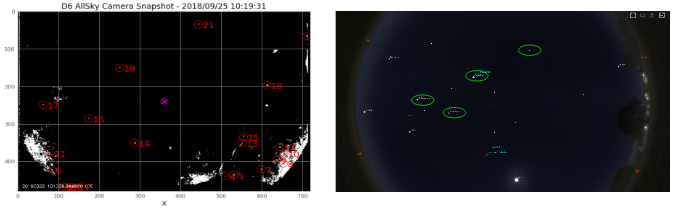
\includegraphics[width=1.0\textwidth]{images/stellarium_sidebyside.png}}
  %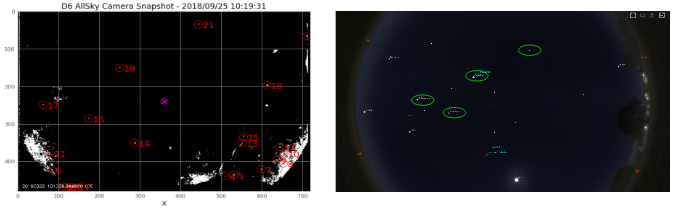
\includegraphics[scale=0.43]{images/stellarium_sidebyside.png}
  \caption{A D6 AllSky snapshot (left) alongside a Stellarium display (right).  We compare the two to find recognized stars that are found in both images.  These are circled in lime green in the Stellarium display. }
  \label{star_recognition}
\end{figure}


Once an object in a given frame is matched to a name, we used the Python library \texttt{Astroquery} and its function \texttt{Vizier} to automatically look up the star's right ascension, declination, V-magnitude, azimuth, and elevation.  
This, combined with the star's pixel location, time, and original snapshot's file name, was added to our star catalog as a singular data row.

\begin{figure}[h]
  \centering
  \includegraphics[scale=0.4]{images/az_el.png}
  \caption{A visualization of altitude and azimuth measurements on a unit sphere.  Note that a positive azimuth angular measurement moves from North towards East.}
  %   \setcaptioncitation{https://en.wikipedia.org/wiki/Horizontal_coordinate_system#/media/File:Azimuth-Altitude_schematic.svg}
  \label{altaz}
\end{figure}

\subsubsection{Azimuth and Elevation}

Each star has several inherent properties such as magnitude, right ascension, and declination.  
The later two represent coordinates that locate a star on the celestial sphere.  
Other properties, such as a star's azimuth and elevation change over time and vary dependent on the observers location.  
These two properties indicate a star's position in the sky relative to an observer and act similarly to spherical coordinates.

Figure \ref{altaz} shows how altitude and azimuth coordinates are determined. 
Note that the azimuth is an angle with respect to North.
A move closer to a pure East direction reflects a positive azimuth angle, whereas a move in the West direction reflects a negative azimuth angle.
Through finding the azimuth and elevation of a star, we can assign a star a 3-D coordinate value that lays on a unit sphere.  
We can then calculate the angular separation between two 3-D coordinates by taking advantage of properties of the dot product:

$$ \vec{A} \cdot \vec{B} = |\vec{A}||\vec{B}| \cos{(\theta)} $$

where $\theta$ represents the angular separation between the two unit vectors.  
Because we know that both vectors representing star locations will fall on a unit sphere, their magnitude is $1$.
Using this knowledge, we may transform the above equation to:

$$ \theta = \arccos{(\vec{A} \cdot \vec{B})} $$

Given this formula we calculate the angular distance that separates two different celestial objects.
The average angular distance per pixel measurement is determined by taking the angular distance divided by the pixel distance between the two celestial objects' pixel locations.
This equation is important and can be seen the following equation:

$$ \textrm{Avg. Angular Distance per Pixel} = \frac{\theta}{\textrm{pixel separation}} $$




\subsection{Calculating Angular Areas}

The D6 AllSky Camera is a versatile system and it's orientation and position can change slightly from night to night.
Because of this, there are several considerations that must be accounted for when calculating angular distance per pixel across different camera regions.
The D6 AllSky Camera is a versatile observation tool, and it therefore takes observations in slightly different locations each time it is put out.
A change in observation location could mean that if one night a star is located at pixel value $(10,10)$, and the next night it could be located at $(94,134)$.
We have developed a method for calculating angular separation per pixel data points that account for this consideration.

\subsubsection{Comparing Objects from the same Night}

The star catalog stores information about celestial objects over the course of all observations.
Using constraints from the Time Analysis information (start time, end time, time elapsed), we can isolate rows within the star catalog from a specific night.  
After creating this subsection, we can then use our described method to calculate the angular separation per pixel for every combination of two objects.
One might question where the data behind this angular distance per pixel should be located.
After all, there are two different object locations used to calculate the value.
Our strategy was to locate the point in between the two objects.  
Figure~\ref{starcombos} depicts these combinations along with the locations of the angular separation per pixel represented as white dots.

\begin{figure}[ht!]
  \centering
  \includegraphics[scale=0.70]{images/star_combinations.png}
  \caption{A set of four stars (yellow) that could be compared to calculate six separate angular distance per pixel data points (white).}
  \label{starcombos}
\end{figure}

Figure~\ref{starcombos} gives a general depiction of our method on a much smaller scale.
Note that when comparing objects from this subsection of the star catalog, we are not limited to only comparing different stars.
As an object moves throughout the night sky, its azimuth and elevation change along with its pixel location.
We can thus treat each individual observation as a unique object, even comparing between the same object at different times throughout the night.
This creates many more combinations than if we were to only consider unique stars.

After calculating all potential angular separation per pixel values alongside their location information, we may move on to calculating average angular separation per pixel in different camera regions.
For the sake of dividing our field of view into different pixel regions, we split up our $720 \times 480$ pixel camera frame into $40 \times 40$ pixel squares.
This also allows us to observe the difference in angular distance per pixel ratios across the entire field of view

\begin{figure}[h]
  \centering
  \makebox[\textwidth][c]{\includegraphics[width=1.0\textwidth]{images/rotated_pixels.png}}
  \caption{Left: our angular separation per pixel data set. Right: that same data set with two rotated and appended data sets.}
  \label{rotate}
\end{figure}


There are $216$ total pixel regions and only so many angular separation per pixel data points.
Some pixel regions that do not contain any data points.
By assuming that our field of view has rotational symmetry, we can rotate and append new data to our set.
Figure \ref{rotate} shows one data set that is rotated twice in $10 \degree$ increments.
For the sake of this project, we rotated our original data $360 \degree$ in $5 \degree$.  
This allowed us to fill in all of the empty regions and multiply our data set quantity by over $50$.
All angular separation per pixel measurements located inside a given square were then averaged over to determine that square's average angular separation per pixel value.

\section{Calculating Cloud Coverage}

The D6 AllSky Camera currently does not always remain outside.
For the most part, our camera was only placed outside during nights where observation conditions were promising.
Because we cannot see or properly analyze fireball events that happen behind clouds, we cannot count cloudy regions as observable areas.
As mentioned previously, the D6 AllSky Camera takes several snapshots of the night sky systematically throughout an observing session.
Specifically, it currently takes images every $30$ minutes.
By using thresholding, we have seen how we can determine which pixels qualify as not observable areas.
The threshold value that we used in this step was a photon value of $90$.


We chose a different threshold pixel value for this cloud analysis than the threshold in our star recognition program.
While thresholding for star recognition, we want to minimize the number of false positives.
The more distinguishable bright small objects in a given frame, (ex: pixels on the edge of a cloud) the larger number of objects that meet our \texttt{SimpleBlobDetector} parameters.
This adds a hefty bulk of time sifting through false positive objects.
While trying to find clouds, we don't want to get rid of hazy cloud boundaries, so we utilize a lower threshold.

Unfortunately, some pixels that fall within a broad cloud area are not recognized through this process.
The solution to this problem lies in the \texttt{OpenCV} functions \texttt{MORPH\_CLOSE} and \texttt{MORPH\_ERODE}.
The first of these functions fills in regions of empty space that are next to filled in space.
This is helpful in closing gaps between pixels that represent clouds.
However, because the edges of the clouds are expanded in this process, we must subsequently perform a \texttt{MORPH\_ERODE} that works in the opposite fashion.
Once a hole is completely closed, there is no space within a cloud for the eroding function to open up, hence providing a satisfying answer to the cloud predicament. 
The difference between a thresholded image and the subsequently closed/eroded image can be seen in the upper-right and lower-left panels of Fig. ~\ref{colorclouds}.
We may observe that this method fills in a vast majority of the small dark holes in the thresholded image.

After this successful threshold and subsequent closing/eroding process is complete, the next step is implementing the relationships between pixels and angular distance.
By assigning the correct regional angular separation per pixel value to each pixel within a cloud, we are able to estimate the angular area that cloud covers.
Figure~\ref{colorclouds} shows the processes taken in calculating the area occupied by clouds.
Note that both a filling and eroding function was used to attain the lower left image.
The observable area during that time is the cloud coverage subtracted from the total observation area.


\begin{figure}[ht!]
  \centering
  \includegraphics[scale=0.4]{images/Cloud_analysis.png}
  \caption[Calculating cloud area coverage from thresholding and applying our angular distance per pixel map.]{From top left to bottom right: a cloudy D6 snapshot, that snapshot with a threshold applied, the thresholded image after a close/erode function was applied, the subsequent pixels assigned angular distance per pixel measurements.  The angular distance per pixel map is discussed more thoroughly in the Data chapter.}
  \label{colorclouds}
\end{figure}

This process is performed for each snapshot.
In creating our average area observed calculations, we assume that the sky retains that same amount of cloud coverage for the $15$ minutes prior to and $15$ minutes after the snapshot.
While this isn't precise down to the exact minute, over many observations, the number of over-estimations and under-estimations should average out and yield an accurate observational area.























 
